\begin{frame}{Le schéma multivarié UOV}
    \large{\centerline{\textbf{Comment faire une (mauvaise) vinaigrette}}}
     \centering
    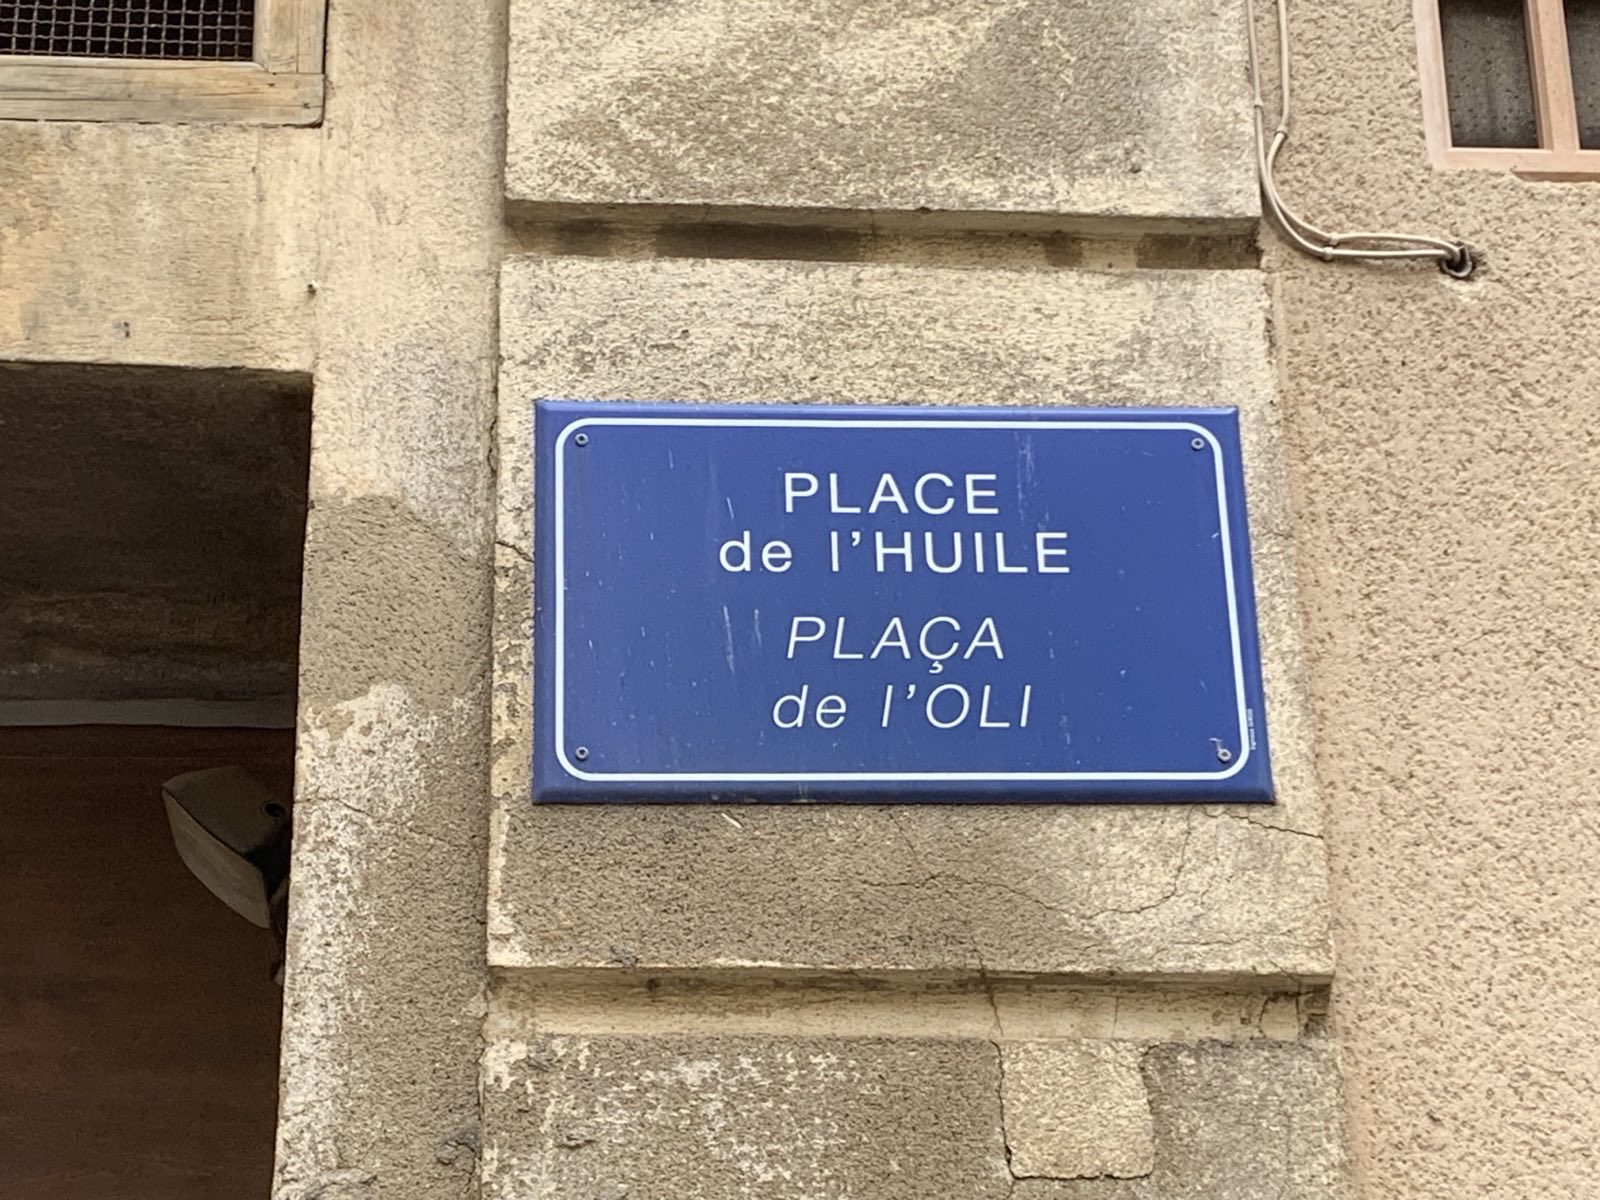
\includegraphics[trim=12cm 8cm 8cm 8cm, clip, width=0.5\linewidth]{img/meme/UOV-vac.jpg}
\end{frame}

%------------------------------------------------
%------------------------------------------------

\begin{frame}{Ça tourne au vinaigre \FiveStar\FiveStar\FiveStar \hfill 9 résolutions}
    \begin{columns}[c]
        \column{.55\textwidth}
        \begin{center}                  
            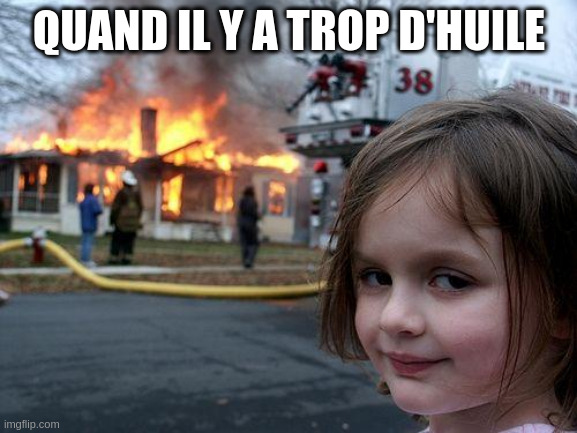
\includegraphics[width=0.9\textwidth]{img/meme/uov-intro.png}
        \end{center}

        \column{.45\textwidth} % 
           \begin{outline}
               \1 Objectifs :
                \2 Forger une signature valide
                \2 Sans la clef privée
                \pause
                \2 \textcolor{red}{Sans la clef publique}
                \pause
               \1 Données :
                    \2 1600 signatures

           \end{outline}
    \end{columns}
\end{frame}

%------------------------------------------------
%------------------------------------------------

%------------------------------------------------
%------------------------------------------------

\begin{frame}{Sur les représentations des fonctions quadratiques}
    \begin{columns}[c]
        \column{.50\textwidth}

            \begin{block}{Fonction quadratique}
                $f(x_1,\dots,x_n) = $
                \only<1>{
                    $\underset{i\leq j}{\displaystyle\sum} a_{ij}x_ix_j$ 
                }
                \only<2->{
                    \colorbox{blue!20}{$\underset{i\leq j}{\displaystyle\sum}a_{ij}x_ix_j$}
                }
                $ + $
                \only<1>{
                    $\underset{i}{\displaystyle\sum} b_{i}x_i$
                }
                \only<2->{
                    \colorbox{red!20}{$\underset{i}{\displaystyle\sum} b_{i}x_i$}
                }
                $ +\, c$
                \only<2->{
                    \\
                    \hspace{2.55cm}
                        \text{\scriptsize\color{blue!60} (quadratique)}
                    \hspace{0.65cm}
                        \text{\scriptsize\color{red!60} (linéaire)}
                }
            \end{block}
            \pause
            \begin{block}{Forme quadratique}             
                $f'(\textbf{x},\textbf{x}) = \underset{i\leq j}{\displaystyle\sum} a_{ij}x_i x_j$ \pause $= \textbf{x}^T \textbf{A} \textbf{x}$
            \end{block}

        \column{.45\textwidth}
            \only<3>{
            \begin{figure}
                \centering
                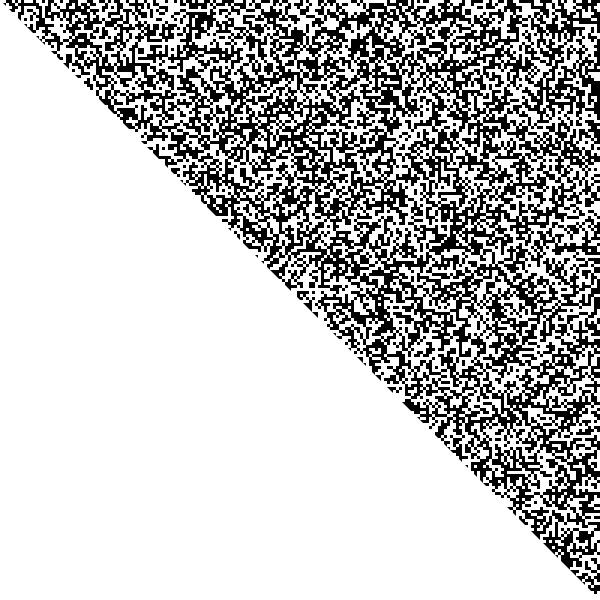
\includegraphics[width=5cm]{img/crypto/UOV/quadratic.png}
                \begin{tikzpicture}[overlay, remember picture]
                \end{tikzpicture}
                \captionsetup{labelformat=empty} % Removes the 'Figure' label
                \caption{Représentation matricielle d'une forme quadratique}

            \end{figure}
            }
            \only<4->{
                \begin{figure}
                \begin{tikzpicture}
                
                    \node[anchor=south west,inner sep=0] (image) at (0,0) {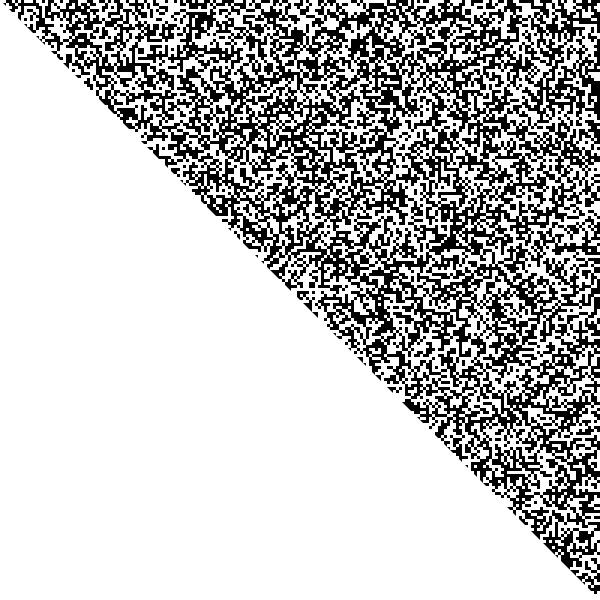
\includegraphics[width=5cm]{img/crypto/UOV/quadratic.png}};
                    \begin{scope}[x={(image.south east)}, y={(image.north west)}]
                        % Adjust these coordinates (0–1 range) to point to your (i,j) coefficient
                        \def\x{0.7}
                        \def\y{0.6}
                        \def\size{0.01}
                
                        % Draw square around pixel
                        \draw[red, line width=1.5mm] (\x-\size, \y-\size) rectangle (\x+\size, \y+\size);
                
                        % Axis labels
                        \node[above=2pt, xshift=\x*5cm, text=red] at (image.north west) {$j$};
                        \node[right=2pt, yshift=\y*5cm, text=red] at (image.south east) {$i$};
                            \node[red, right=\x*2.5cm, yshift=\y*2.5cm] {$a_{ij}x_ix_j$};
                    \end{scope}
            \end{tikzpicture}
            \captionsetup{labelformat=empty} % Removes the 'Figure' label
            \caption{Représentation matricielle d'une forme quadratique}
            \end{figure}
        }
    \end{columns}

\end{frame}

\begin{frame}{Sur les formes bilinéaires}

$f(x_1,\dots,x_n) = \underset{i\leq j}{\displaystyle\sum} a_{ij}x_ix_j + \underset{i}{\displaystyle\sum} b_{i}x_i + c$
    \begin{block}{Forme bilinéaire}             
        $f'(\textbf{x},\textbf{y}) = \underset{i\leq j}{\displaystyle\sum} a_{ij}x_i y_j$ \pause $= \textbf{x}^T \textbf{G} \textbf{y}$ \pause \hfill $/!\backslash$ $\textbf{}G$ est de taille maximale
    \end{block}
    \pause
    \begin{itemize}
        \item Pour $\textbf{y}$ fixé, une équation en $\textbf{x}$ est linéaire (et vice versa)
    \end{itemize}
    \pause
    \begin{block}{Composition}
        $f'(\textbf{x},\textbf{y})=f(\textbf{x}+\textbf{y})-f(\textbf{x}) - f(\textbf{y})+f(\textbf{0})$ est une forme bilinéaire symétrique
    \end{block}

    \begin{itemize}
      \item  Les parties linéaires et constantes se simplifient
      \item $(\textbf{x}+\textbf{y})^T \textbf{A}(\textbf{x}+\textbf{y}) = \textbf{x}^T\textbf{A}\textbf{x}+\textbf{y}^T\textbf{A}\textbf{y}+\textbf{x}^T(\textbf{A}+\textbf{A}^T)\textbf{y}$
    \end{itemize}
    
\end{frame}

\begin{frame}{Une signature via UOV (Unbalanced Oil and Vinegar)}
    
    \begin{block}{La clef publique UOV}
        $\mathcal{Q}=(\mathcal{Q}_1,\dots,\mathcal{Q}_h)$ des fonctions quadratiques à n variables

        $\mathcal{Q}_i(\textbf{y}) = \textbf{y}^T\textbf{A}_i\textbf{y} + \textbf{b}_i^T\textbf{y} + c_i $
    \end{block}
    \pause
    La signature de $\textbf{t}=(t_1,\dots,t_h)$ est une solution $\textbf{y}=(y_1,\dots,y_n)$ du système $\mathcal{Q}(\textbf{y})=\textbf{t}$ :
    \[\left\{
    \begin{array}{c}
       \mathcal{Q}_1(\textbf{y}) =  \mathcal{Q}_1(y_1,\dots,y_n) = t_1 \\
       \vdots \\
       \mathcal{Q}_h(\textbf{y}) =  \mathcal{Q}_h(y_1,\dots,y_n) = t_h \\
    \end{array}
    \right.\]
    \pause
    \begin{block}{Difficulté du problème UOV}
        Pour des bonnes valeurs de $h$, $v$ et $n=h+v$ , il est difficile de résoudre un tel système quadratique quelconque.
    \end{block}
    \pause
    Sans clef privée, il est difficile de signer un message
\end{frame}

\begin{frame}{La trapdoor d'UOV}
$\mathbb{F}_q^n=\mathbb{F}_q^h \oplus\mathbb{F}_q^v = \mathcal{H}\oplus\mathcal{V}$ (huile + vinaigre) $\pause \Rightarrow$ $\textbf{x} =(x_1,\dots,x_h,x_{h+1},\dots,x_{h+v}) = (\mathbf{x}_\mathcal{H},\mathbf{x}_\mathcal{V})$
    \pause
    \begin{columns}
        \column{.45\textwidth}
            \begin{figure}
                \begin{tikzpicture}
                
                    \node[anchor=south west,inner sep=0] (image) at (0,0) {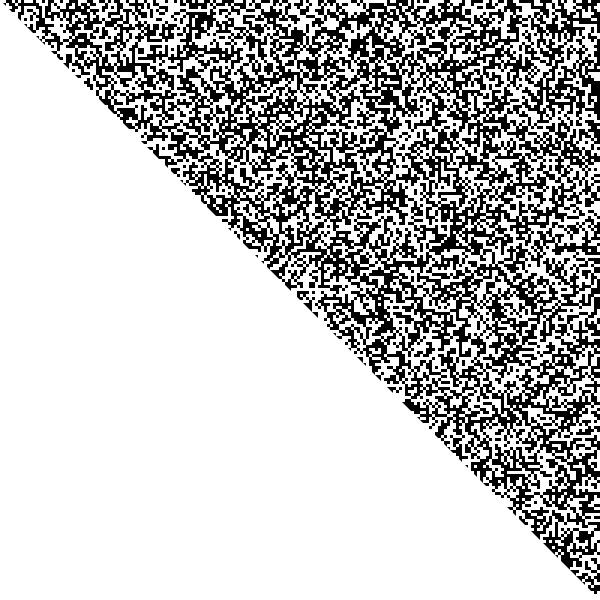
\includegraphics[width=3cm]{img/crypto/UOV/quadratic.png}};
                    \begin{scope}[x={(image.south east)}, y={(image.north west)}]
                        % Adjust these coordinates (0–1 range) to point to your (i,j) coefficient
                        \def\x{0.7}
                        \def\y{0.6}
                        \def\size{0.01}
                
                        % Draw square around pixel
                        \draw[red, line width=1.5mm] (\x-\size, \y-\size) rectangle (\x+\size, \y+\size);
                
                        % Axis labels
                        \node[above=2pt, xshift=\x*3cm, text=red] at (image.north west) {$j$};
                        \node[right=2pt, yshift=\y*3cm, text=red] at (image.south east) {$i$};
                            \node[red, right=\x*1cm, yshift=\y*1cm] {$a_{ij}y_iy_j$};
                    \end{scope}
            \end{tikzpicture}
            \captionsetup{labelformat=empty} % Removes the 'Figure' label
            \caption{Partie quadratique de $\mathcal{Q}_i$ publique}
            \end{figure}
        \pause
        \column{.05\textwidth}
        $\overset{\mathbf{y}=\mathcal{S}(\mathbf{x})}{\Leftarrow}$
        \column{.45\textwidth}
            \begin{figure}
                \begin{tikzpicture}
                
                    \node[anchor=south west,inner sep=0] (image) at (0,0) {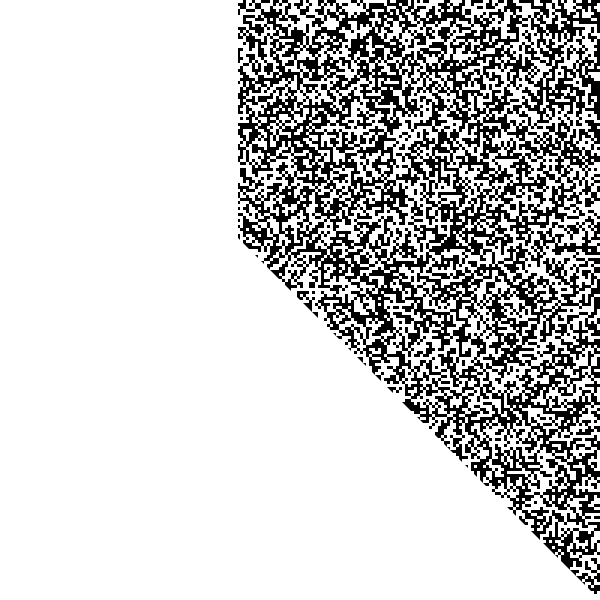
\includegraphics[width=3cm]{img/crypto/UOV/trapdoor.png}};
                    \begin{scope}[x={(image.south east)}, y={(image.north west)}]
                        % Adjust these coordinates (0–1 range) to point to your (i,j) coefficient
                        \def\x{0.25}
                        \def\y{0.8}
                        \def\size{0.2}

                        \only<5->{
                            % Draw square around pixel
                            \draw[red, line width=1.5mm] (\x-\size, \y-\size) rectangle (\x+\size, \y+\size);
                    
                            % Axis labels
                            \node[red, right=\x*0cm, yshift=\y*1cm] {\shortstack{$a'_{ij}=0$ \\ pour $i,j<h$}};
                        }
                    \end{scope}
            \end{tikzpicture}
            \captionsetup{labelformat=empty} % Removes the 'Figure' label
            \caption{Partie quadratique de $\mathcal{P}_i=\mathcal{Q}_i\circ \mathcal{S}$ privée}
            \end{figure}
    \end{columns}
    \pause
    \begin{itemize}
        \item Par construction, $\mathcal{P}_i(\mathbf{x})=\mathcal{P}_i((\mathbf{x}_\mathcal{H},\mathbf{x}_\mathcal{V}))$ est \textit{linéaire} en $\mathbf{x}_\mathcal{H}$ pour $\mathbf{x}_\mathcal{V}$ fixé.
        \pause
        \item Pour $\mathbf{x}_\mathcal{V}$ fixé, il est trivial de résoudre $\mathcal{P}(\mathbf{x}_\mathcal{H},\mathbf{x}_\mathcal{V})=\mathbf{t}$
        \pause
        \item Pour $\mathbf{y}=\mathcal{S}(\mathbf{x})$ sera une solution valide de $\mathcal{Q}(\mathbf{y}) =\mathbf{t}$
    \end{itemize}
    
\end{frame}

\begin{frame}{Récapitulatif d'UOV}
    \pause
    \begin{block}{Keygen}
        \begin{itemize}
            \item Générer un changement de variable linéaire $\mathcal{S}$ aléatoire (matrice $n\times n$)
            \pause
            \item Générer $\mathcal{P}_{i<h}$ quadratique tels que $\mathcal{P}_i((\mathbf{x}_\mathcal{H},\mathbf{x}_\mathcal{V}))$ est linéaire en $\mathbf{x}_\mathcal{H}$ pour $\mathbf{x}_\mathcal{V}$ fixé
            \pause
            \item \textbf{Clef publique} : $\mathcal{Q} = \mathcal{P}\circ \mathcal{S}^{-1}$ avec  $h{{n+1}\choose{2}}$ coefficients 
            \pause
            \item \textbf{Clef privée} : $\mathcal{P}$, $\mathcal{S}$ avec $h\left({{n+1}\choose{2}}-{{h}\choose{2}}\right)$ et $n^2$ coefficients 
        \end{itemize}
    \end{block}

    \pause
    \begin{block}{Signature de $m$}
        \begin{itemize}
            \pause
            \item Encoder $m$ comme $\mathbf{t}\in\mathbb{F}_q^h$
            \pause
            \item Fixer aléatoirement $\mathbf{x}_\mathcal{V}\in\mathcal{V}$
            \pause
            \item Résoudre $\mathcal{P}((\mathbf{x}_\mathcal{H},\mathbf{x}_\mathcal{V}))=\mathbf{t}$ (linéaire en $\mathbf{x}_\mathcal{H}$). Si pas de solution, choisir un autre $\mathbf{x}_\mathcal{V}$
            \pause
            \item \textbf{Signature}: $\mathbf{y} = \mathcal{S}(\mathbf{x})$ est une solution du système $\mathcal{Q}(\mathbf{y}) =\mathbf{t}$
        \end{itemize}
    \end{block}
\end{frame}

\begin{frame}{Retour au challenge}
    \begin{block}{Parametres}
        \begin{itemize}
            \item $n=60$, donc polynômes à 60 variables, vecteurs $\mathbf{x}$, $\mathbf{y}$ de dimensions 60 
            \item $h=24$, donc 24 équations quadratiques $\mathcal{P}_i$ et $\mathcal{Q}_i$
            \item $v=n-h=36$, donc 36 variables de $\mathbf{x}_\mathcal{V}$ à fixer pour la signature
        \end{itemize}
    \end{block}

\pause
\vspace{0.6cm}

    \begin{outline}
        \1 Analyse du code source
    \end{outline}

            \begin{columns}
                \column{.45\textwidth}
                \begin{tcolorbox}
                    \begin{minipage}{\columnwidth}
    \textbf{Keygen}: La clef privée inverse $h$ et $v$ (au lieu d'avoir 24 inconnues linéaires dans la clef privée, on en a 36)
                    \end{minipage}%
                \end{tcolorbox}
                \pause
                \column{.45\textwidth}

                \begin{tcolorbox}
                    \begin{minipage}{\columnwidth}
    \textbf{Signature}: les 36 valeurs de $\mathbf{x}_\mathcal{V}$ sont déterministes, calculées via SHAKE256 du message, donc connues
                    \end{minipage}%
                \end{tcolorbox}

            \end{columns}       
\end{frame}

\newcommand{\vin}{\mathcal{V}}
\newcommand{\hui}{\mathcal{H}}
\renewcommand{\S}{{\mathcal{S}}}
\newcommand{\sV}{{\mathcal{S}_{|\vin}}}
\newcommand{\sH}{{\mathcal{S}_{|\hui}}}

\newcommand{\xV}{\mathbf{x}_\vin}
\newcommand{\xH}{\mathbf{x}_\hui}
\newcommand{\yV}{\mathbf{y}_{\vin'}}
\newcommand{\yH}{\mathbf{y}_{\hui'}}



\begin{frame}{Sur la confidentialité des vecteurs vinaigres \footnote{\cite{cryptoeprint:2023/1131}}}

    \pause 

    $\mathbf{\k{y}}=\S(\mathbf{\u{x}})=\S(\k{\xV})+\S(\u{\xH})=\sV(\k{\xV})+\sH(\u{\xH})$ car $\mathbb{F}_q^n =\vin\oplus \hui$ 

    Avec $\sV:\vin\longrightarrow \S(\vin):=\vin'$ et $\sH:\hui\longrightarrow \S(\hui):=\hui'$ des \textit{isomorphismes}
    
    \vspace{0.4cm}
    \pause 
    
       Ceci donne $\sV^{*}(\mathbf{\k{y}}) = \mathbf{\k{x_\vin}} + 0$ \pause $\longrightarrow$ On interpole $\sV$ donc $\vin'$ avec $36*60/36=60$ signatures

    \vspace{0.4cm}
    \pause
    Comme $\mathcal{P}$ est linéaire sur $\hui$, après changement de variable $\mathcal{Q}=\mathcal{P}\circ \S$ sera linéaire sur $\hui'$

    \begin{block}{Forger une signature UOV}
         $\mathbb{F}_q^n =\vin' + \hui'$, donc connaître l'espace $\vin'$ ou $\hui'$ suffit à forger une signature UOV
    \end{block}

%    Ainsi $\hui'\bigcap\vin' = \{0\}$ et donc $\sV^{-1}\circ\sH = 0$

    \vfill
   \pause

   On a toujours pas la clef publique...
\end{frame}

\begin{frame}{Récupérer la clef publique}
On a 1600 signatures :
    \begin{outline}
        
        \1 Interpolation polynomiale de la clef publique $\u{\mathcal{Q}_i}: \k{\mathbf{y}} \mapsto \k{\mathbf{t}_i}$ 
            \2 ${{n+1}\choose{2}}=1891$ inconnues pour chaque $\u{\mathcal{Q}_i}$ \pause $\rightarrow$ n'exploite par la connaissance de $\vin'$

        \pause
        
        \1 Interpolation polynomiale de la clef privée, $\u{\mathcal{P}_i} : \k{\xV} \oplus \u{\xH} \mapsto \k{\mathbf{t_i}}$
            \2 $\left({{n+1}\choose{2}}-{{h}\choose{2}}\right)=1591$ inconnues par $\u{\mathcal{P}_i}$ \pause $\rightarrow$ chaque $\u{\xH}$ rajoute des inconnues
    \end{outline}

        \pause
    \[
        \begin{tikzpicture}[baseline=(eq.base)]
            \node (eq) at (0,0) {$\u{\mathcal{Q}_i}(\mathbf{\k{y}})=\u{\mathcal{Q}_i}(\k{\yV}+\k{\yH})=\u{\mathcal{Q}_i}(\k{\yV})+\u{\mathcal{Q}_i}(\k{\yH})+\u{\mathcal{Q}'_i}(\k{\yV},\k{\yH})-\u{\mathcal{Q}_i}(\mathbf{0})$};
            \foreach \x/\label in {
                -1.3/\only<6->{${37}\choose{2}$ \tiny{[quad]}},
                0.45/\only<6>{${25}\choose{2}$ \tiny{[quad]}} \only<7->{\textbf{25 \tiny{[linear]}}},
                 2.15/\only<6->{$24\cdot36$  \tiny{[biquad]}},
                 4.7/\only<6->{$1$  \tiny{[const]}}
            } {
                \only<6->{\draw[<-, thick] (\x,-0.25) -- ++(0,-0.4) node[below] {\scriptsize \label};}
            }
            \node (tot) at (-4,-0.9) {\footnotesize{\only<6>{1893 inconnues} \only<7->{\textbf{1593} inconnues}}};
        \end{tikzpicture}
    \]
    \only<8->{
        On a donc assez de signatures pour interpoler les $\mathcal{Q}_i$ \hfill \flag
    }
\end{frame}